\chapter{Implementation}
\label{chp:implementation}
This chapter explains how the hybrid vehicle, which is similar to the Toyota Prius second generation, was modelled in Simulink. Then the implementation details in Matlab of each of the six game-theoretical approaches are described.

\section{Hybrid Vehicle Model}
The model of the hybrid vehicle is split into different controllers and each of them is responsible for controlling the corresponding part of the hybrid. The chapter describes the Drive Cycle Controller, the Power Controller, the Gasoline Engine Controller, the Electric Motor Controller, the Transmission and the Vehicle Dynamics. The game-theoretical logic is included in the Power Controller, which is the principal controller where the solution is computed. It is shown in the next section.

\subsection{Drive Cycle Controller}
This subsection deals with the demand of speed which comes from the Drive Cycle and how it is transformed to acceleration demand, which corresponds to the acceleration pedal in a vehicle.

Two different drive cycles were simulated. The FTP-75 drive cycle is intended to test light-duty vehicles in the U.S. and measure their gas emissions and fuel economy. It lasts for 1874s, the total distance it covers is 17.77km and the average speed is 34.1 km/h. The drive cycle contains three phases - cold start from 0-504s, transient phase from 505-1369s and hot start from 1370-1874. The last phase is exactly the same as the first phase. Figure \ref{fig:ftp75} shows the time and speed of this drive 
cycle.

\begin{figure}[h]
\centering
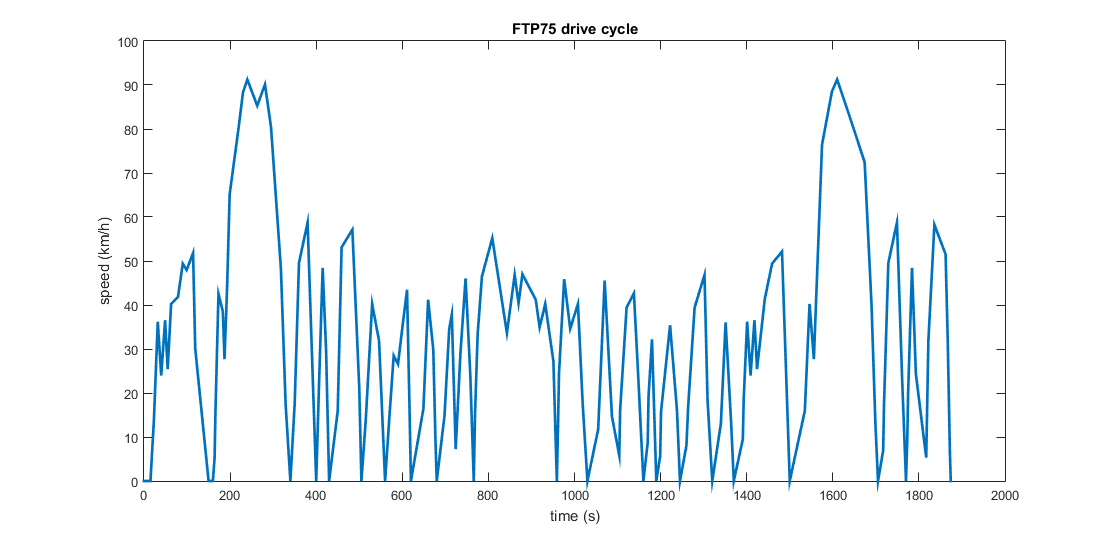
\includegraphics[scale=0.45]{figures/FTP75}
\caption{FTP drive cycle}
\label{fig:ftp75}
\end{figure}

The NEDC drive cycle was invented to test light-duty cars in Europe. Its duration is 1180s, the distance is 11.02km and the average speed 33.6km/h. It contains four equivalent urban driving phases called ECE-15. They last from 0-780s and there is also a fourth highway driving phase called EUDC from 781-1180s. Figure \ref{fig:nedc} shows the time versus the speed in the NEDC drive cycle.

\begin{figure}[h]
\centering
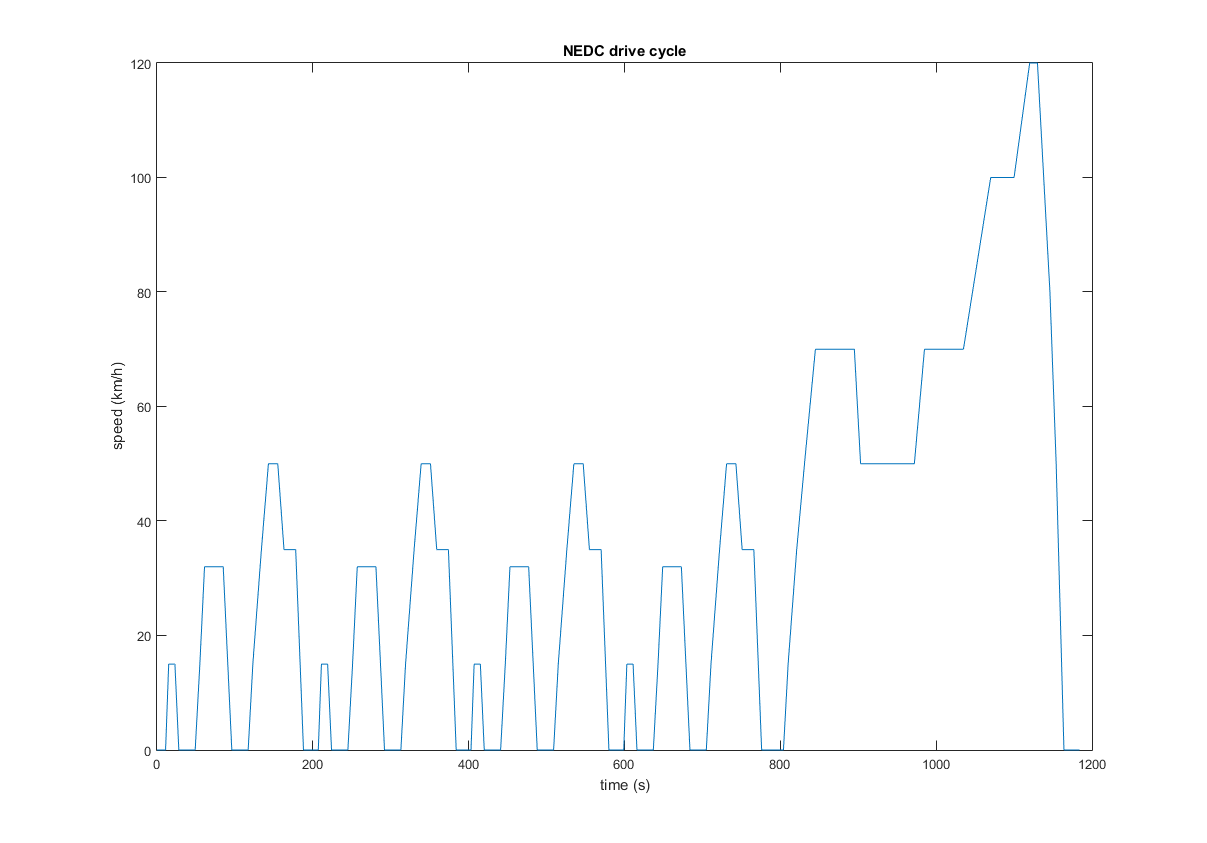
\includegraphics[scale=0.45]{figures/NEDC}
\caption{NEDC drive cycle}
\label{fig:nedc}
\end{figure}

The Speed Control block takes as input the demanded speed from the drive cycle and the actual speed of the vehicle both in \textit{km/h} and calculates as output the acceleration which lies between -1 and 1 where a negative value means braking and a positive value means acceleration. A value of 0 corresponds to cruising or maintaining a constant speed. In order to calculate the acceleration demand, the difference between the demanded and actual speed is taken.

\subsection{Power Controller}
The Power Controller takes as input the acceleration demand $a$ and the state of charge $SOC$ of the battery which comes from the Electric Motor Controller. In order to transform the acceleration demand into torque demand $\tau_{dem}$, the acceleration is scaled by the maximum torque of 400 \textit{Nm} which can be requested. This value was chosen since this is the maximum output torque of the Toyota Prius electric motor. The minimum demanded torque is -400 \textit{Nm} which corresponds to deceleration. The current motor speed $\omega_{mot}$ is mapped to the torque of the motor which it is capable of generating at this moment. This value is taken as upper limit and its negated value is taken as a lower limit of the torque. 

There are two subsystems in the Power Controller, the Battery Management and the Game Theory Controller. The first of them takes as input the battery $SOC$, its current in \textit{A}, its voltage in \textit{V} and computes the required recharge power $P_{batReq}$ and the battery limit $P_{batLim}$. The recharge power is requested when the SOC of the battery lies between 40 and 60\%. If the SOC falls below 40\% then the battery is forced to be recharged even if that means not meeting the drive cycle requirements and not achieving the demanded speed. After the battery has been charged up to 60\%, the recharging stops and the requested battery power is set to 0. The battery limit calculation takes into account that the maximum voltage of the battery is 200V and that its maximum power is 21 kW.

The Game Theory Controller is the primary place where the computation of the solution to the power distribution problem happens. The outputted demanded torque $\tau_{dem}$ is fed into the Game Theory Controller block. In addition, the other inputs of this block are required power, which is:
\begin{equation}
P = \tau \times \omega
\end{equation}
where power $P$ is in \textit{W}, torque $\tau$ is in \textit{Nm} and the velocity $\omega$ is angular \textit{rad/s}.
The Game Theory Controller also receives the battery SOC in \%, the generator $\omega_{gen}$, engine $\omega_{eng}$, motor $\omega_{mot}$ speeds all in \textit{rad/s}, the Total Fuel consumed up to this moment from the beginning of the drive cycle $TF$ in \textit{litres}, the battery limit and the required battery recharge power $P_{batReq}$ as described in the Battery Management subsystem above. The Game Theory Controller block contains the game-theoretical logic embedded as a Matlab function. Apart from it, it also regulates the speed of the engine by taking the difference between the required driving power $P_{drive}$ and the recharge power for the battery $P_{batReq}$. The resulting power is given as an input to a lookup table to find the corresponding engine speed in \textit{rpm}. To obtain the Generator torque $\tau_{gen}$ the engine torque and the generator speed $\omega_{gen}$ in \textit{rad/s} are taken. If the motor needs to provide additional power for the battery, this power is taken to be the sum of the battery available power and the generator power. The battery available power $P_{batAv}$ is computed in a separate subsystem using the engine torque $\tau_{eng}$, speed $\omega_{eng}$ and power $P_{eng}$, battery recharge power $P_{batReq}$ and battery limit $P_{batLim}$. 
Four values come as a result from the Game Theory Controller, the engine throttle $\theta$, the motor torque $\tau_{mot}$, the generator torque $\tau_{gen}$, the reference engine speed in \textit{rpm} $\omega_{eng}$. These are fed to a final Speed Controller block for controlling the engine speed which outputs the final engine throttle $\theta$ as percentage from the maximum possible torque of the engine $\tau_{engMax}$.

\subsection{Engine Controller}
The Engine Controller receives the throttle in \% as input and sends the torque as output. The Gasoline Engine library block implements a gasoline fuel engine and its speed controller. Firstly, the masked library block and then the extensions added to it to will be explained.

In the Gasoline Engine block the input signal between 0 and 1 indirectly controls the engine speed. Whenever the input is outside of the allowed range it is limited to 0 or 1 respectively. The mapping of speed in \textit{rpm} to torque in \textit{Nm} is implemented by a lookup table. The throttle goes through a Switch block which ensures that the maximum speed of the engine is not exceeded. If this happens, the throttle is set to 0. Otherwise the torque and the angular velocity are measured and after that the torque flows to the output. The angular velocity measured in \textit{rad/s} is fed back to the lookup table in \textit{rpm} to find the corresponding torque and it is also given to the switch block for controlling the maximum speed.

An additional functionality which was implemented to extend the library block was to limit the torque from 0 to 136 and also speed from 0 to 6000 rpm. Figure \ref{fig:engineTorqueSpeed} shows the torque speed curve of the engine. It provides maximum torque of 135 to 136 in the speed range 2800 - 3200 rpm. For this reason when the acceleration is constant and the engine provides maximum torque, there is a discrepancy in the simulation results, because the speed keeps jumping from 2800 to 3200 quickly, which is inefficient. Therefore, a hysteresis was implemented by a Relay block which has a switch on and a switch off point values. When the signal lies between 2800 and 3200 rpm it is either set to 2800 or to 3200 rpm to prevent such jittering.

A Driveline environment is connected to the output of the Gasoline Engine block which provides the simulation environment. In addition, attaching a Torsional Spring-Damper \citep{tsdMatlab} allows the torque to flows between two rotating axes, the base and the follower. The input (base) is connected to the output of the Gasoline Engine library block which is the torque, whereas the output (follower) is grounded using an Housing block to prevent it from rotating. The Torsional Spring-Damper takes as parameters the stiffness (spring rate) set to 0 \textit{N*m/rad} and the damping (kinetic friction) set to 0.2079 \textit{N*m*s/rad}. The torque depends on the relative displacement angle and relative angular velocity. Moreover, the outputted torque from the Gasoline Engine block has another connection to an Inertia block, which acts as a rigid rotating body. Torque and angular velocity are measured and given along with the throttle to a Scope block for displaying the results of the engine. Power is also calculated by taking the product of torque and velocity.

A separate subsystem is responsible for the fuel and gas emissions calculations. It receives the engine speed in \textit{rpm} and the torque and outputs Total Fuel $TF$ in \textit{l}, Fuel Consumption $FC$ in \textit{l/100km}, CO emissions, HC emissions, NOX emissions all in \textit{g/km}. In order to calculate them lookup tables are applied, which hold the data for the gas emissions in grams per second \textit{g/s}. To transform \textit{g/s} into \textit{g/km} the total distance travelled is required. That is why the average speed of the drive cycle is calculated and is multiplied with the total time. 

\subsection{Electric Motor Controller}
The Electric Motor Controller is a large subsystem containing the battery, a DC/DC converter, the motor and the generator. It receives as input the demanded motor torque and generator torque. It outputs the battery characteristics and the actual motor torque and actual generator torque.

The battery is modelled by a Battery block of a Nickel-Metal-Hydride type. The nominal voltage is 200V and the rated capacity is 6.5Ah. At the beginning of the simulation the battery is fully charged, its state of charge is set to 100\%. The discharge characteristics are shown in Figure \ref{fig:batteryDischarge}. The first figure shows the nominal discharge current and the second shows the discharge curves at the specific discharge currents. The discharge model $f_1$ and charge model $f_2$ of the battery are \citep{batteryMatlab}:

\begin{equation}
\begin{split}
f_1(it,i*,i,Exp) = E_0 - K \cdot \frac{Q}{Q-it} \cdot i* - K \cdot \frac{Q}{Q-it} \cdot it + Laplace^{-1} \bigg( \frac{Exp(s)}{Sel(s)} \cdot 0 \bigg)
\end{split}
\end{equation}

\begin{equation}
\begin{split}
f_2(it,i*,i,Exp) = E_0 - K \cdot \frac{Q}{|it|+0.1 \cdot Q} \cdot i* - K \cdot \frac{Q}{Q-it} \cdot it + Laplace^{-1} \bigg( \frac{Exp(s)}{Sel(s)} \cdot \frac{1}{s} \bigg)
\end{split}
\end{equation}
where $E_0$ is the constant voltage, $Exp(s)$ is the exponential zone dynamics in $V$, $Sel(s)$ is the battery mode, 0 for discharging and 1 for charging, $K$ is polarization constant in $Ah^{-1}$, $i*$ is the low frequency current dynamics in $A$, $i$ is the battery current in $A$, $it$ is the extracted battery capacity in $Ah$, $Q$ is the maximum battery capacity in $Ah$.

The DC/DC converter is directly attached to the battery. Its purpose is to convert direct current from one voltage to another, from the battery voltage to the motor and generator voltage. The DC bus voltage of the whole electric system is maintained at 500V. 

The Electric Motor subsystem is modelled similar to the AC6 - 100 kW Interior Permanent Magnet Synchronous Motor (PMSM) Drive library model \citep{ac6Matlab}. The motor is a PMSM as in the Toyota Prius. However, the implemented model in this thesis is a 50 kW instead of 100 kW and the bus voltage is 500VDC instead of 288VDC like in the AC6 library model. In total there are four main parts of the electric motor - the PMSM, the Three-phase Inverter, the VECT controller and the Speed Controller. 

The inputs of the Motor block are torque in \textit{Nm}, enable 0 or 1, speed in \textit{rad/s} and the plus and minus from the battery. The outputs are the three motor characteristics - stator current in \textit{A}, rotor speed in \textit{rad/s}, electromagnetic torque in \textit{Nm} and the speed control containing the reference torque in \textit{Nm}. The Speed controller receives as input the speed and an Enable signal. The incoming torque is converted to speed using a lookup table and fed into the Speed controller. It outputs the torque and transmits it to the VECT controller, whose output are three reference line currents. They are given to the Three-phase converter which converts voltage. The Simulink library block Permanent Magnet Synchronous Machine \citep{pmsmMatlab} is used for the implementation of the motor itself. On this motor there are 8 poles and the rotor is of type salient-pole, which means that the magnets are buried. It is a three-phrase motor and has a sinusoidal back electromotive force EMF. The mechanical input can either be the torque \textit{Nm} or the speed in \textit{rad/s}, but in this case it is the speed. Depending on the sign of the torque coming as input the block can either work as a motor or as a generator. When the sign is positive it operates as a motor and if it is negative, it acts as a generator. 

The motor's characteristics are plotted in the Electric Motor scope. These include the current in \textit{A}, the rotor speed \textit{rpm}, the measured and the reference torque \textit{Nm} and also the power in \textit{W}. The outputted torque from the motor is limited between -400 and 400 \textit{Nm} and is also used as output from the whole Electric Motor Controller.

The Generator block is modelled in the exact same manner as the Motor block. Again the Simulink block Permanent Magnet Synchronous Machine \citep{pmsmMatlab} is utilized. Nevertheless, the generator is a 30 kW machine in contrast to the 50 kW motor. The minimum and maximum torque are the same as in the motor, -400 and 400 \textit{Nm} and are limited within this range using a Saturation block. The generator's resulting stator current in \textit{A}, rotor speed in \textit{rpm}, measured and reference torque in \textit{Nm} and power in \textit{W} are displayed in the Generator scope.

\subsection{Transmission}
The main purpose of the transmission or the gearbox is to incorporate the torque from the engine, motor and generator and to transmit the combined torque to the vehicle. In the Toyota Prius this transmission system is called the Power Split Device (PSD). 

The Transmission subsystem receives as input the torque from the engine, motor and generators. The output is the combined torque of these three which flows into the Vehicle dynamics subsystem where it is transmitted to the wheels. The transmission consists of a planetary gear with a carrier, ring and sun gears. Each of these three gears is connected to one source of torque. The engine is connected to the planetary carrier, the motor is attached to the ring gear and the generator to the sun gear. After merging the torques they are outputted from the ring, where the motor is attached. While the axle of the carrier and thus rotates the ring and sun gears using the inside planet gears, the ring gear axle transmits the torque to the wheels in the Vehicle model. The sun gear's axle, where the generator is attached, is responsible for converting the power of the engine to electrical energy.

The Planetary gear block itself is implemented by the model in \citet{planetMatlab}. It consists of one planet-planet gear and one ring-planet gear. The parameter ring/sun gear ratio is fixed and is set to 2.6. When the sun rotates in one direction, the ring co-rotates in the other direction with regard to the carrier gear and vice versa. This gear ratio $g_{RS}$ also corresponds to the number of teeth in the ring and sun gear and to the torque ratio between them $g_{RS} = N_R/N_S = \tau_R/\tau_S$. There are two geometry constraints regarding the radii of the gears. The radius of the carrier is the sum of the radius of the sun and planet gears $r_C = r_S + r_P$, whereas the radius of the ring gear is the sum of the carrier radius and the planet radius $r_R = r_C + r_P$. In addition, there are two kinematic constraints which say that $r_C\omega_C = r_S\omega_S + r_P\omega_P$ and $r_R\omega_R = r_C\omega_C + r_P\omega_P$. This means that the angular velocity of the carrier is the sum of the velocities of the sun and planet gear and the angular velocity of the ring is the sum of the carrier and planet velocities.

In the Transmission subsystem there are three scopes which show simulation results. The first scope is about torque and displays the three torques of the carrier, ring and the sun all in \textit{Nm}. The second scope is the speed scope showing the angular velocity in \textit{rad/s} of the carrier, sun and ring. Lastly, the power scope shows sun, ring and the carrier power in \textit{W} which should be the sum of the ring and sun power.

\subsection{Vehicle dynamics}
The last subsystem models the vehicle dynamics. It receives as input the combined torque which is coming from the motor port, where all three torques of the motor, engine and generator are merged. The torque is measured with a Torque sensor, whose output is connected to a Torsional Spring-Damper. The parameters stiffness and damping are set to 0 \textit{N*m/rad} and 0.1 \textit{N*m*s/rad} respectively. A Simple Gear block \citep{simpleGearMatlab} transfers the torque. The block is a gearbox consisting of two axes, a base and a follower, which rotate with a fixed ratio of 4.113 in this case. Whenever the sign of the two axes is the same, they rotate in the same direction and when it is different, they rotate in opposite directions. An Inertia block with 0.5 $kg*m^2$ is attached to the torque output of the Simple Gear before it goes to the differential. 

The Differential block as in \citet{differentialMatlab} represents a differential gear which receives a longitudinal axis as input and sends two lateral axes as output. Usually the two lateral axes rotate with distinct angular velocities. A single parameter is necessary for the Differential block and that is the  drive gear ratio $g_D$, in this case 1. It predetermines the relationship $\omega_B = \frac{1}{2} \cdot g_D(\omega_{F1} + \omega_{F2})$ between the longitudinal base axis $\omega_B$ and the two lateral axes $\omega_{F1}$ and $\omega_{F2}$. Either of the following two cases can be true. Firstly, the longitudinal shaft is the same as the two lateral shafts when they rotate with the same velocity $\omega_{F1} = \omega_{F2}$. Secondly, the longitudinal shaft can be locked, $\omega_B = 0$ when the lateral shafts rotate in the opposite direction $\omega_{F1} = -\omega_{F2}$. The last constraint is that the input and output power of the differential must be the same: $\omega_B \tau_B = \omega_{F1} \tau_{F1} + \omega_{F2} \tau_{F2}$.

Each of the two output shafts of the differential is connected to one inertia block with 0.5 $kg*m^2$. The left and right tires are modelled with the Tire block \citep{tireMatlab}. It requires the following parameters - effective rolling radius of 0.3 \textit{m}, rated vertical load 3000 \textit{N}, peak longitudinal force at rated load 3500 \textit{N}, slip at peak force at rated load 10\% and relaxation length at rated load 0.2 \textit{m}. The inputs of the Tire block are $V_x$ and $F_z$, where $V_x$ is the wheel longitudinal velocity in \textit{m/s} and $F_z$ is the vertical load in \textit{N}. The outputs are $\Omega$, which is the wheel angular velocity expressed in \textit{rad/s} and $F_x$ is the longitudinal force in \textit{N}. Figure \ref{fig:tire} shows how these forces are applied on the wheel.

\begin{figure}[h]
\centering
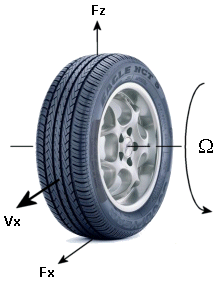
\includegraphics[scale=0.8]{figures/tire}
\caption{Forces affecting the tire \citep{tireMatlab}}
\label{fig:tire}
\end{figure}

Each of the two tires is connected to the primary block in the Vehicle Dynamics subsystem. This is the Longitudinal Vehicle Dynamics \citep{vehicleDynMatlab}, which implements the dynamics of a vehicle with two axles and four wheels. Its inputs are the incline angle $\beta$ and the front and rear longitudinal forces $F_{xf}$ and $F_{xr}$, which come from each of the front and rear tires' outputs $F_x$. The block produces as outputs the vehicle velocity $V_x$ and also the vertical load forces for the front and rear tires $F_{zf}$ and $F_{zr}$. These two are transmitted to the $F_z$ input ports of the wheels. In addition, the block calculates the vehicle velocity which is also fed back to the wheels' ports $V_x$. Before sending the output of the whole Vehicle Dynamics subsystem, the speed is transformed from \textit{m/s} to \textit{km/h}.

\section{Game-theoretical algorithms}
This chapter deals with the implementation of all six game-theoretical approaches in Matlab. Firstly, a description of the initialization and the parent function, which calls each of the solutions and that is embedded in the Simulink model, is given. Then, each function for the game theory solution is explained in detail.

\subsection{Initialization functions}
\label{sec:initfunc}
Before starting the simulation, the environment has to be prepared by initializing variables. The initialization function is called \textit{prepare.m} and it calls the functions for preparing the fuel, exhaust emissions and drive cycle data. 

Firstly, the fuel consumption rate lookup table is explained. The data comes from \citet{argonne1999} where a Toyota Prius first-generation model was tested. Nevertheless, due to lack of any newer publicly available reports which state the results of torque-speed relationship and the corresponding fuel consumption and gas emissions, this data is utilized. The fuel data is read from a file, which contains the engine speed in \textit{rpm}, torque in \textit{Nm}, fuel consumption rate in \textit{gal/s} and engine power in \textit{kW}.  A conversion between \textit{gal/s} to \textit{g/s} is done by:
\begin{equation}
gps = \frac{galps * 719.7 * 1000}{264.172}
\end{equation}
where 719.7 * 1000 $g/m^3$ is the density of gasoline and 264.172 $gal/m^3$ converts $gal$ to $m^3$. After the conversions the minimum and maximum speed, torque, fuel consumption rate and power are given to the Matlab \textit{linspace} function in order to generate linearly spaced vectors of size 10 for each of the inputs. Then the function \textit{meshgrid} is applied to produce a grid from the input vectors of torque and speed. The torque and speed are also passed to two \textit{fit} functions, once with the fuel consumption rate and once with the power in order to fit a polynomial surface to the data. Moreover, the fuel and power consumption surface is plotted. For this purpose a polynomial function has to be chosen. Experimentation was done with different polynomial curves like poly22, poly23 and finally poly22 was chosen. The first 2 corresponds to the degree in x and the second 2 or 3 corresponds to the degree in y. Finally, the fuel consumption rate and the power lookup tables are created by the function \textit{feval} which takes the fuel and power fit and evaluates the function at the grid points, returned by the meshgrid function. The resulting 3D plots are shown in Figure \ref{fig:fuelFit} and Figure \ref{fig:powerFit}.

The second initialization step is to generate the exhaust emissions lookup tables. The data also comes from \citet{argonne1999} and is read from a file. Exactly the same procedure with the \textit{linspace}, \textit{meshgrid}, \textit{fit}, \textit{feval} functions like in the fuel consumption rate above is applied. The resulting fits of the CO, HC and NOX emissions are shown in Figures \ref{fig:coFit}, \ref{fig:hcFit} and \ref{fig:noxFit}.

Lastly, the final step is to prepare the drive cycle data of FTP75 and NEDC. The FTP75 data is read from a file, which has two columns, the first is the time in seconds and the second is the speed in miles per hour. The \textit{mph} are converted to \textit{km/h} by multiplication with 1,60934. Since the drive cycle's duration is 1874s, it is split into 5 different phases, so that simulation can be simplified in case any errors occur and the whole drive cycle has to be started again. The splitting points were selected so that every phase starts and ends with a demanded speed of 0 \textit{km/h}. The following table shows the duration of each of the five phases:

\begin{table}
\centering
\begin{tabular}{ |c|c|c| } 
 \hline
 Drive cycle phase & Start (s) & End (s) \\
 \hline\hline
 FT75-1 & 0 & 340 \\ 
 FT75-2 & 341 & 680 \\ 
 FT75-3 & 681 & 1030 \\ 
 FT75-4 & 1031 & 1500 \\ 
 FT75-5 & 1501 & 1874 \\ 
 \hline
\end{tabular}
\caption{Drive Cycle splitting in 5 phases}
\end{table}

\subsection{Embedded Matlab function in Simulink}
The Matlab function, incorporated in the Simulink model, is responsible for calculating the payoff functions and afterwards calling all other game-theoretical solutions.
The inputs it receives are the required torque in \textit{Nm}, the State of Charge (SOC) of the battery in \% and the fuel consumed in $l$ at this time step. In addition, it takes two lookup tables, containing the data of the fuel consumption and gas emissions. Any required torque between 0 and 83, which is the minimum torque that the engine can produce, is automatically passed only to the motor. No game has to be played, since the engine is incapable of providing such a small amount of torque. Negative required torque is also directly attributed to the motor only, because the engine is also unable to provide negative torque. During torque demands less than 0, the battery is recharged and the motor is transforming the mechanical energy to electric energy and sending it to the battery. Therefore, only when the torque demand lies within the range 83-400, a game-theoretical solution is computed.

\subsubsection{Strategies computation}
A crucial parameter, which influences the performance of the whole embedded function and thus the whole computation time of the simulation, is the number of pure strategies for each player during the game. A value of 7 is chosen to be the number of strategies after experimenting with values between 5 and 15. For 15 strategies the computation times becomes too large and there is not a big difference to the solution with 7 strategies; hence, the smaller number 7 was chosen.

The strategies represent how much torque the engine and the motor contribute and this is expressed as \% of the required torque or of the maximum torque they are capable of generating. Therefore, the maximum motor and engine strategies are taken to be the minimum of two values - required torque and maximum engine/motor torque. Then, the engine and the motor strategies are computed by the \textit{linspace} Matlab function, which creates a linearly spaced vector between two values with a specific length, in this case 7. Consequently, 0\%, 16.66\%, 33.32\%, 49.98\%, 66.64\%, 83.3\%, 100\% of the required torque are taken as the strategies. For the motor these two minimum and maximum values of the vector are 0 and the required torque respectively, since the motor can produce any torque between 0 and 400, which is also the maximum torque that can be requested. For the engine these two values are 83 (its minimum torque capability) and either the required torque or 136 (maximum torque capability), whichever is smaller. To illustrate this with an example, if the required torque is 120, then the strategies of the motor will be 0, 19.99, 39.98, 59.97, 79.96, 99.95 and 120 \textit{Nm}. The strategies of the engine will be 83, 89.16, 95.32, 101.48, 107.64, 113.8, 120 \textit{Nm}. 

\subsubsection{Payoff computation}
The payoff function of the motor is computed as shown in Equation \ref{eq:payoffMotor}. Each of the components of the payoff has a different weight. After conducting experiments, the following weights were established: $w_1 = w_{FCR} = 3$ for fuel consumption rate, $w_2 = w_{TD} = 0.5$ for torque deviation, which corresponds to fulfilling the driver demands, $w_3 = w_{HC} = 45$ for HC emissions, $w_4 = w_{CO} = 25$ for CO emissions, $w_5 = w_{NOX} = 65$ for NOX emissions, $w_6 = w_{TF} = 0.5$ for accumulated total fuel consumed to this moment.
The payoff function of the engine is also implemented as in Equation \ref{eq:payoffEngine}. The respective weights are $w_7 = w_{PC} = 0.5$ for the power consumed by the motor and the $w_8 = w_{SOC} = 1$ is for the battery SOC deviation from the target 70 \%.

The payoff matrix of the engine is of size $m \times n$. The calculation of each component in the payoff function is explained in detail next. In order to calculate the fuel consumption rate in \textit{g/s} a 2D lookup table of size $10 \times 10$ is utilized. For a given torque and speed of the engine, it outputs the fuel consumption rate. In order to find the closest value to the engine strategy from all 10 torque values in the lookup table, the minimum absolute difference between all 10 torque values and the engine strategy is taken. To find the engine speed, an interpolation between the torque and speeds values at the specific point of the engine strategy is required. Then, when the torque and the engine speed, corresponding to this torque, are known they are given to the fuel consumption table to find the fuel consumption rate. The torque deviation is computed as the absolute difference between the required torque and the total torque (sum of the motor and engine strategies). After that, the gas emissions are the next components in the payoff function. The same torque and corresponding engine speed are used as inputs to the CO, NOX and HC emissions lookup tables, which work in the same manner as the fuel consumption lookup table.

Similarly, the engine payoff is also a $10 \times 10$ matrix. The calculation of the first component in this payoff function, the torque deviation, was explained above. The power consumed by the motor in $kW$ is computed according to:
\begin{equation}
P = \frac{\tau \times v}{9,5488 \cdot 1000}
\end{equation}
where the velocity is in \textit{rpm} and thus the factor 9,5488 is needed to convert it to \textit{rad/s} and 1000 is for obtaining the power in $kW$ instead of $W$. The SOC deviation is computed by taking the absolute difference between the 70 \% target, which is the charged capacity that the battery tries to maintain, and the SOC at this time step. This deviation can at most be 30 \% and this happens when the battery is fully charged at 100 \% or when the battery is charged at its minimum allowed charge state of 40 \%. The battery SOC must not fall below this percentage. If this happens, a recharging process immediately starts even if the driver demands cannot be met any more.

With this the description of the payoff function is finished. The next subsection explains the game-theoretical approaches implementation in Matlab.

\subsection{Pareto Efficiency}
Implementation of the Pareto Efficiency is done in the function \textit{paretoset.m}. Firstly, this function receives the payoff of the engine and motor in two variables. All outcomes in both payoff matrices are examined in order. For each payoff it is checked whether there exists another payoff with a smaller engine payoff (x-coordinate) and a smaller motor payoff (y-coordinate). If that is the case, then the current payoff is not a Pareto outcome and a flag is set. If after checking all outcomes against the current outcome there is still no smaller payoff for both players, then this is regarded as a Pareto efficient outcome. Furthermore, it is verified that another outcome with a difference of at most 0.000001 from the current outcome is not already saved in the Pareto efficiency vector. The function outputs the set of Pareto efficient payoffs in a matrix where each row holds the x and y values of the Pareto outcome. In addition, the indices of the Pareto efficient points inside the payoff matrices are returned in the same way.

\subsection{Pareto Optimality}
Due to the fact that there can be more than one Pareto efficient points, a criteria has to be defined in order to choose a single point to be the solution. This single solution or Pareto Optimality is implemented in the function \textit{bestpareto.m}. The function takes as input the outputs of the \textit{paretoset.m} function and additionally the torque deviation, the fuel consumption rate and the motor power. Three different criteria are defined regarding the choice of the solution point. First of all, the point with the smallest absolute torque deviation is taken as the Pareto optimal point. In case that the size of the vector returned by this minimum absolute difference is bigger than 1, or when there are more than one such points, then a second criterion is applied. Thus, the point with the minimum fuel consumption rate is taken. Again, if the size of the returned vector is bigger than 1, a third criterion is exploited. The point with the minimal power, consumed from the motor, is taken as final solution. As output the function returns a pair of x and y coordinates of the Pareto optimal solution payoff.

\subsection{Nash Equilibrium}
The algorithm for finding Nash Equilibrium, the Lemke-Howson algorithm, was explained thoroughly in Subsection \ref{subsec:lemkehowson}. There are various algorithms for computing Nash Equilibria, for example, the \textit{NPG} Matlab function as described in \citet{npg}. However, this function is too slow in comparison with the Lemke-Howson function \citep{lemkeHowson2014Matlab}. Therefore, it was decided not to use the \textit{NPG} function at all. The Lemke-Howson function takes as input the two payoff matrices of the engine and motor and the initial pivot $k$. The pivot is the starting label to drop, as already explained in Subsection \ref{subsec:lemkehowson}. Since there are $m+n$ labels (strategies) which can be dropped first and they can end up in a different Nash Equilibrium node in the graph, it is inefficient to experiment with all different starting strategies. Experiments were done with $1$, $\frac{m+n}{4}$, $\frac{m+n}{2}$, $\frac{3(m+n)}{4}$ and $m+n$ as the first strategy to be dropped. In order to decide which number to use, the Matlab function NPG is run. The Lemke-Howson solution with the $k$-th strategy, which is closest to the NPG solution is chosen, $k = \frac{m+n}{2}$ and it is passed as input to the Lemke-Howson algorithm, whose detailed implementation will not be explained. In principle, it is implemented as a complementary pivoting algorithm for bimatrix games. Originally it returns the mixed strategy Nash Equilibrium in a pair of two cell arrays, one for each player's mixed strategy distribution. Nevertheless, cells are not supported in code generation for the Simulink model. Therefore, the algorithm was slightly altered so that it returns the pair of payoffs which represent one Nash Equilibrium in normal arrays instead of cells.

\subsection{Nash Bargaining Solution}
The next solution approach, the Nash bargaining solution is implemented in the function \textit{nashsolution.m}. It takes as input one matrix of size $2 \times (m*n)$, where the first column is the engine payoff, whose matrix is transformed to a vector, and the second columns is the motor payoff. The function also requires as input the conflict point, which is taken to be the Nash Equilibrium point, produced by the Lemke-Howson algorithm. The algorithm works by going over the whole payoff pairs and computing the Nash Product by the formula in Equation \ref{eq:nashProduct}. In the end, the payoff pair with the maximum Nash product is taken to be the Nash bargaining solution. The output of the function is the maximized Nash product and the index of the Nash Solution pair.

\subsection{Kalai-Smorodinsky Solution}
The Kalai-Smorodinsky bargaining solution is implemented in the function \textit{kalaismorodinsky.m}. It takes as arguments the same matrix containing both player's payoffs as column vectors, the conflict point like in the Nash solution, the Pareto payoff strategies and their indices. It returns the payoff pair of the Kalai-Smorodinsky solution.

Firstly, the function finds the ideal point, which is often an infeasible point because it is the minimum of both payoffs. Since the Kalai-Smorodinsky solution is defined as the intersection point of the ideal and conflict points with the Pareto Frontier line, an interpolation between the ideal and conflict points is required. To interpolate between the two values it must be checked whether there are repeated x or y values which can impede the function \textit{interp1} by causing an error. If there are duplicate x values, then interpolation along the y values is performed and if there are duplicate y values vice versa. 

Furthermore, interpolation between all Pareto efficient point has to be done in order to get all points on the line segments connecting the Pareto efficient points. Then, the closest point to the exact intersection point is taken. Since there can be more than two Pareto points, all of them need to be sorted either according to x or to y values. An interpolation from the smaller to the larger coordinates is done by using the function \textit{linspace} and \textit{interp1}. The linearly spaced vector created between any two Pareto points contains 100 points. This number is chosen since a large number is needed in order to accurately find the closest interpolated point to the real point. However, an even larger number than 100 will be too space-consuming and does not necessarily increase the accuracy when the two points' x or y coordinates differ only slightly, for instance, just with 1 or 2. The interpolation is applied to the first and second points, then to the second and third and so on until all Pareto efficient points are connected. Afterwards, the Kalai-Smorodinsky solution is computed by equalizing the ratios as in Equation \ref{eq:kalaismorodinsky}. For all points on the line segments, connecting all Pareto efficient payoffs, it is tested whether the two ratios of the x and y coordinates - between the conflict point with the point on the Pareto Frontier and between the conflict point with the ideal point, are the same. Prevention of division by zero is also taken into account. Nevertheless, it can happen that the left and right sides of Equation \ref{eq:kalaismorodinsky} are never equal, because the interpolation has not produced exactly the same point as the real intersection point, but rather a point with a very small difference in the second or third decimal places. Therefore, the difference between the right and left hand-sides of each interpolated point on the Pareto Frontier is computed so that if this case occurs, the point with the minimum absolute difference is taken as the Kalai-Smorodinsky solution.

The function returns the pair of payoffs for the Kalai-Smorodinsky solution. Often the point does not coincide exactly with a payoff pair from the input payoff matrices; hence, the solution is not feasible in pure strategies. In this case the function additionally returns the two Pareto efficient points, between which the Kalai-Smorodinsky solution lies, and their indices. The reason is that these two Pareto points are later utilized to compute a mixed strategies solution.

Whenever randomization between between the two Pareto points by computing mixed strategies is necessary, probabilities are assigned to both Pareto strategies in the following way. It is assumed that the two Pareto points $u_1$, $u_2$ are sorted in descending order so that the $u_1$ is bigger in x and y than $u_2$. It is further assumed that x coordinates correspond to the engine or player 1 and y coordinates correspond to the motor or player 2. Let us denote the Kalai-Smorodinsky point with $ks$. There are three cases according to which the probabilities of the two strategies are computed. Firstly, when the x and y coordinates of both Pareto efficient points are different, then the ratio $P(s_1) = \frac{ks(x) - u_1(x)}{u_2(x) - u_1(x)}$ is taken to be the probability of $u_1$'s strategy $s_1$. The probability of $p_2$'s strategy $s_2$ is similarly $P(s_2) = \frac{ks(y) - u_2(y)}{u_1(y) - u_2(y)}$. Secondly, when the x coordinates of $u_1$ and $u_2$ are the same, then the ratios of the y coordinates are taken. For the second strategy the probability is again $P(s_2) = \frac{ks(y) - u_2(y)}{u_1(y) - u_2(y)}$ and for the first strategy it is $P(s_1) = 1 - P(s_2)$. Thirdly, when the y coordinates of $u_1$ and $p_2$ are the same, the ratios of the x coordinates are computed. Therefore, $P(s_1) =  \frac{ks(x) - u_1(x)}{u_2(x) - u_1(x)}$ and $P(s_2) = 1 - P(s_1)$.

The payoffs of the two mixed strategies are computed as follows:
\begin{equation}
s_1 = u_1(x) + P(s_1)(u_2(x) - u_1(x))
\end{equation} 

\begin{equation}
s_2 = min(u_1(y), u_2(y)) + P(s_2)|u_1(y) - u_2(y)|
\end{equation}
In the end the torques of the engine $\tau_1$ and the motor $\tau_2$ corresponding to the strategy payoffs are calculated as follows:
\begin{equation}
\tau_1 = min(s_1(x), s_2(x)) + P(s_1)|s_1(x) - s_2(x)|
\end{equation}
\begin{equation}
\tau_2 = min(s_1(y), s_2(y)) + P(s_1)|s_1(y) - s_2(y)|
\end{equation}

\subsection{The Core}
Computation of the core requires finding all imputations. For this reason coalition payoff matrices have  to be calculated and this happens in the function \textit{coalitionpayoffs.m}. It receives the payoffs of the engine and motor, the torque deviation $\delta_{tau}$ and a linearly spaced vector $\tau$ from 0 to the required torque, which is of size 10. For instance, if the required torque is 108, then the vector  $\tau = \{0,12,24,36,48,60,72,84,96,108\}$. The idea of coalition payoffs is to modify the original payoff matrices so that the smaller the torque deviation is, the smaller the modified payoff becomes and therefore the more optimal. This is achieved by multiplication with the so called coalition coefficients, which vary from 0.99 to 1 within steps of 0.001. Therefore, torque deviation of 0 \textit{Nm} corresponds to the smallest coalition coefficient of 0.99. Negative torque deviation from $-\tau(2) < \delta_{\tau} < 0$ has coefficient 0.991, from $ 0 < \delta_{\tau} < \tau(2)$ has 0.992 and so on until $\tau(9) < \delta_{\tau} < \tau(10)$ where it is 1.0. After the coalition payoffs are computed, the engine and motor payoffs are multiplied with the coefficients and the two resulting matrices are added to get the final grand coalition payoffs. The function \textit{coalitionpayoffs.m} returns the modified engine, motor payoffs, the coalition coefficients and the grand coalition payoff. 

The next step for computing the core is to extract the imputations from all allocations. The function \textit{checkimputation.m} takes as arguments the original payoffs of the engine and motor, the modified engine and motor payoffs as column vectors, the grand coalition payoffs matrix and in addition the Pareto efficient payoffs. Since an imputation is always Pareto efficient when it fulfils the condition for Group Rationality as described in \ref{subsec:core}, it is sufficient to only extract the imputations from the Pareto efficient allocations. All Pareto efficient payoffs are examined and for each of them it is verified that no other Pareto payoffs dominates it and that it is individually rational. Domination means that there is no other payoff that is smaller and individual rationality is conformed to when the player receives a smaller payoff in the coalition than when they act alone. The function returns the imputation payoffs and their indices.

In the end, the function for computing the core \textit{core.m} can be called with imputation payoff allocation. The function goes over all imputations and checks whether both players achieve a smaller payoff in the coalition than on their own like in Equation \ref{eq:core}. If this is the case, then the imputation also belongs to the core of the game. As output the function returns the indices of the core allocations.

\subsection{Shapley Value}
\label{subsec:shapleyimpl}
The last game-theoretical approach to be implemented, the Shapley Value, requires an additional transformation of the game space. Although all previous solution approaches work with the strategic form of the game, the Shapley Value cannot be computed solely from the strategic form, but rather calls for a coalitional form. The core also demanded the value of the coalitions, but these values are in matrix form and the coalition payoffs were computed by element-wise multiplication of the payoff matrix of the engine and motor with the coalition coefficients. In addition, for the grand coalition the sum of the two new engine and motor coalition payoff matrices was taken. However, these matrix forms are not sufficient for the Shapley Value. Rather, a single value is needed for each of the three coalitions - player one coalition, player two coalition and the grand coalition, denoted as $v(\{1\})$, $v(\{2\})$ and $v(\{1,2\})$ respectively. The value of the grand coalition is already available, because it is the minimum sum of both players' payoff matrices $v(\{1,2\}) = min(A+B)$. However, the first two values of the individual coalitions are more complex to find, because it is possible that there is no solution in pure strategies and hence no value. It is essential that the values of the two resulting games are computed. In the first game the coalition is individual and includes only the first player, the engine, while in the second game the individual coalition contains only the second player, the motor. That is why the strategic form of the game has to be transformed to coalitional form by finding the characteristic function. According to \citet{ferguson2014game} the value of the resulting game is equivalent to the Saddle point as described in \ref{subsec:shapleyfund}. When no Saddle point exists, thus no solution in pure strategies, mixed strategies have to be computed.

The function which computes the value of the two individual coalitions is \textit{value.m} and takes as input the payoff of one player and the number of that player. The output is a vector with probabilities for each strategy of size $m$ for player 1 or $n$ for player 2. The function is called once for the engine and once for the motor. Firstly, it is tested whether there exists a Saddle point by checking if there is a payoff $u_i$ which is simultaneously a row minimum and a column maximum: $min(max(u_i)) == max(min(u_i'))$. If there is such a payoff point, then in the vector this strategy is marked with probability 1 and all other probabilities are 0. Otherwise, mixed strategies have to be employed. 

Extending the strategy space to mixed strategies involves assigning probabilities to every pure strategy. This problem can be solved by a system of linear equations such that if the engine payoff matrix is the one shown in Table \ref{tab:payoffEngine} and the motor payoff matrix is in Table \ref{tab:payoffMotor}, then the linear system of equations is constructed in the following way. The system can be solved by linear programming (LP) which is a method for minimizing or maximizing a linear objective function, depending on inequality and equality constraints. Furthermore, the function is constrained subject to lower and upper bounds. The Matlab function is called \textit{linprog} and is invoked by \textit{x = linprog(f,A,b,Aeq,beq,lb,ub)}. The purpose is to minimize the function $f$ subject to the constraints:

\begin{equation}
\min_x f^Tx ; \left\{
                \begin{array}{ll}
                  A \cdot x \leq b,\\
                  Aeq \cdot x = beq,\\
                  lb \leq x \leq ub
                \end{array}
              \right.
\end{equation}

The first argument $f$ is the function to be minimized. $A$ is the matrix containing the left side of the system of linear inequalities, whereas $b$ is the right hand-side of this system. Generally, $Aeq$ is also a matrix with the left hand-side of the system of linear equations and $beq$ is the corresponding left-hand side of the system. Since in our case we only have one equation, $Aeq$ is a vector and $beq$ is a scalar. Moreover, as optional arguments lower an upper bounds can be specified which are the vectors $lb$ and $ub$. The last column of $A$ is added to fulfil the constraint that the probabilities of all pure strategies have to sum up to 1. To summarize, only $A$ is a matrix, as shown in Table \ref{tab:A} and all other arguments are vectors except for $beq$ which is a scalar.

$f = [0, 0, 0, 0, 0, 0, 0, -1]$ \\
$lb = [0, 0, 0, 0, 0, 0, 0, -Inf]$ \\
$b = [0, 0, 0, 0, 0, 0, 0]$ \\
$Aeq = [ 1, 1, 1, 1, 1, 1, 1, 0 ]$ \\
$beq = 1$

\begin{table}[h]
\centering 
\begin{tabular}{ |m{0.5cm}|m{0.5cm}|m{0.5cm}|m{0.5cm}|m{0.5cm}|m{0.5cm}|m{0.5cm}|m{0.5cm}| } 
\hline
 $a_{1,1}$ & $a_{1,2}$ & $a_{1,3}$ & $a_{1,4}$ & $a_{1,5}$ & $a_{1,6}$ & $a_{1,7}$ & 1 \\ \hline
 $a_{2,1}$ & $a_{2,2}$ & $a_{2,3}$ & $a_{2,4}$ & $a_{2,5}$ & $a_{2,6}$ & $a_{2,7}$ & 1 \\ \hline
 $a_{3,1}$ & $a_{3,2}$ & $a_{3,3}$ & $a_{3,4}$ & $a_{3,5}$ & $a_{3,6}$ & $a_{3,7}$ & 1 \\ \hline
 $a_{4,1}$ & $a_{4,2}$ & $a_{4,3}$ & $a_{4,4}$ & $a_{4,5}$ & $a_{4,6}$ & $a_{4,7}$ & 1 \\ \hline
 $a_{5,1}$ & $a_{5,2}$ & $a_{5,3}$ & $a_{5,4}$ & $a_{5,5}$ & $a_{5,6}$ & $a_{5,7}$ & 1 \\ \hline
 $a_{6,1}$ & $a_{6,2}$ & $a_{6,3}$ & $a_{6,4}$ & $a_{6,5}$ & $a_{6,6}$ & $a_{6,7}$ & 1 \\ \hline
 $a_{7,1}$ & $a_{7,2}$ & $a_{7,3}$ & $a_{7,4}$ & $a_{7,5}$ & $a_{7,6}$ & $a_{7,7}$ & 1 \\ \hline
\end{tabular}
\caption{ matrix $A$ - left hand-side of system of inequalities}
\label{tab:A}
\end{table}

The function produces a vector $X$ containing the solution of the linear system of equations. The vector has length $m+1$ or $n+1$, the number of strategies, depending on whether the function is called for player 1 or player 2. The first $m$ or $n$ numbers of the vector contain the probabilities of each strategy and they must all add up to 1. The last number in the vector is the solution of the last equation where the column is with all of the 1's as in \ref{tab:A}. That is also the value of the game, corresponding to the individual coalition formed from the player. After the function \textit{value.m} is ran two times for both players, the values of the games are finally available and can be passed to the Shapley value function.

The function \textit{shapleyvalue.m} takes three arguments - the value of the grand coalition, the value of the coalition of player 1 only and the value of the coalition of player 2 only, written as $v_{1,2}$, $v_1$, $v_2$. Then, according to Equation \ref{eq:shapley} the Shapley value of the engine is $\frac{1}{2} (v_{1,2} - v_2) + \frac{1}{2} v_1$ since there is one player in the coalition, $k = 1$ and the total number of players is two, $n = 2$. Similarly, the Shapley value of the motor is $\frac{1}{2} (v_{1,2} - v_1) + \frac{1}{2} v_2$.

Although the two Shapley values are computed, it is often the case that the paoyff they constitute is not feasible in pure strategies. When this occurs, two payoffs or two strategy combinations $t_1, t_2$ have to be found, whose combination in mixed strategies gives the Shapley value payoff $s$. In order to find the two nearest payoff points $u_1$ and $u_2$, the Matlab function $knnsearch$ is utilized to find the K nearest neighbours of the Shapley value, where K is set to 2. Let a variable $i=\{1,2\}$ take values of either 1 or 2. If the two x coordinates of the two nearest payoffs are different, then the x values can be compared or $i=1$, otherwise the y values are compared and $i=2$. There are three possibilities for the Shapley value, either it lies within the range $s_2(i) < s < s_1(i)$ or within $s_1(i) < s < s_2(i)$ or it is smaller than both of them, $s < p_1(i), s < p_2(i)$. In the first case the probability of the first closest payoff is $P(u_1) = \frac{s - u_2(i)}{u_1(i)-u_2(i)}$. In the second case it is $P(u_1) = \frac{s - u_1(i)}{u_2(i)-u_1(i)}$. In the third case the probability depends on whether $u_1$ or $u_2$ is bigger. When $u_1 < u_2$ the probabilities are $P(u_1) = \frac{s}{u_1(i)}$ $P(u_2) = 1 - P(u_1)$ and vice versa for $u_2 < u_1$ they are $P(u_1) = \frac{s}{u_2(i)}$ $P(u_2) = 1 - P(u_1)$. The final step is to compute the engine and motor torque by combining the probabilities of the two closest strategies.

With this implementation description the last solution approach, the Shapley value, the Implementation chapter is finished. The next chapter deals with the Simulation of the whole game-theoretical behaviour.